Для каждого изображения вклад микролинзирования уникален и не зависит от других изображений. Именно эта уникальность и вносит неопределенность в определение временных задержек между изображениями. Для количественных оценок точности определения временных задержек $\Delta t$ и относительных усилений $\Delta m$ между двумя кривыми блеска с учетом микролинзирования разработан следующий подход. За основу была взята одна из кривых блеска SN Refsdal, рассчитанных в гидродинамической модели в различных частотных фильтрах для 400 дней (в системе отсчёта наблюдателя) с момента её взрыва (\cite{petrnat2020}). Она изображена на Рисунке \ref{fig:lightcurves}. 

\begin{figure}[H]
    \centering
	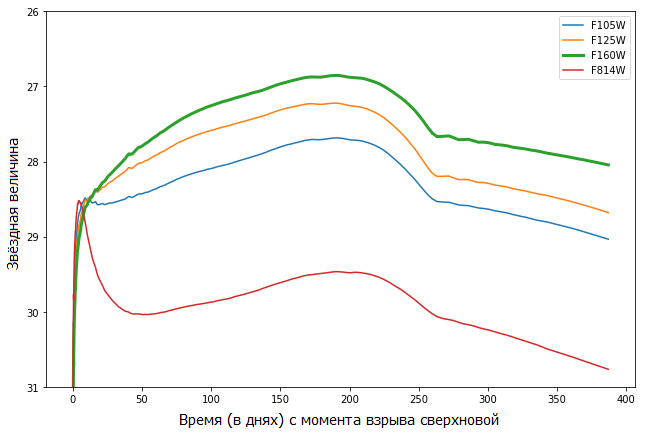
\includegraphics[width=0.79\textwidth]{pics/lightcurves.png}
	\caption{Кривые блеска SN Refsdal в различных фильтрах (HST), полученные в результате гидродинамического моделирования предсверхновой (\cite{petrnat2020}). По горизонтальной оси отложено время в системе отсчёта наблюдателя.} 
	\label{fig:lightcurves}
\end{figure}

Для простоты анализа рассматривается кривая блеска только в одном фильтре -- F160W. Предполагается, что выбранная выше кривая блеска наблюдается в изображении S1 начиная с момента времени $t_0=20$ дней. Для временных интервалов вводится равномерная сетка: частота отсчёта (\textit{cadence}) составляет $5$ дней. Модельная кривая блеска линейно интерполируется по этим точкам. Для имитации изображения S2 эта кривая блеска дублируется и сдвигается по времени на величину $\Delta {t_{21}}^{true}$ и звёздной величине на $\Delta {m_{21}}^{true}$. Значения этих величин ранее были представлены в Таблице \eqref{tab:dtdmpetrnat} и заимствованы из статьи \cite{petrnat2020}:
$${\Delta t_{21}}^{true} = 9.5 \ \textrm{дней}, \ \ \ {\Delta m_{21}}^{true} = -0.14 \ \ \ (\mu_{21} = 1.14)$$

Полученные кривые блеска изображены на Рисунке \ref{fig:lc} на левой верхней панели. Затем к кривым блеска в различных изображениях прибавляются по 50 уникальных для каждого изображения флуктуаций. Рассмотрим одну из таких реализаций (Рис. \ref{fig:lc}, правая верхняя панель). При помощи пакета \texttt{emcee} (\cite{emcee}) методами Монте-Карло с марковскими цепями кривая блеска в изображении S1 аппроксимируется кривой в изображении S2, сдвигаемой по времени и звездной величине: 

$$ m_{S1}^{fit} = m_{S2}(t - \Delta t)-\Delta m. $$ 

\begin{figure}[H]
    \centering
	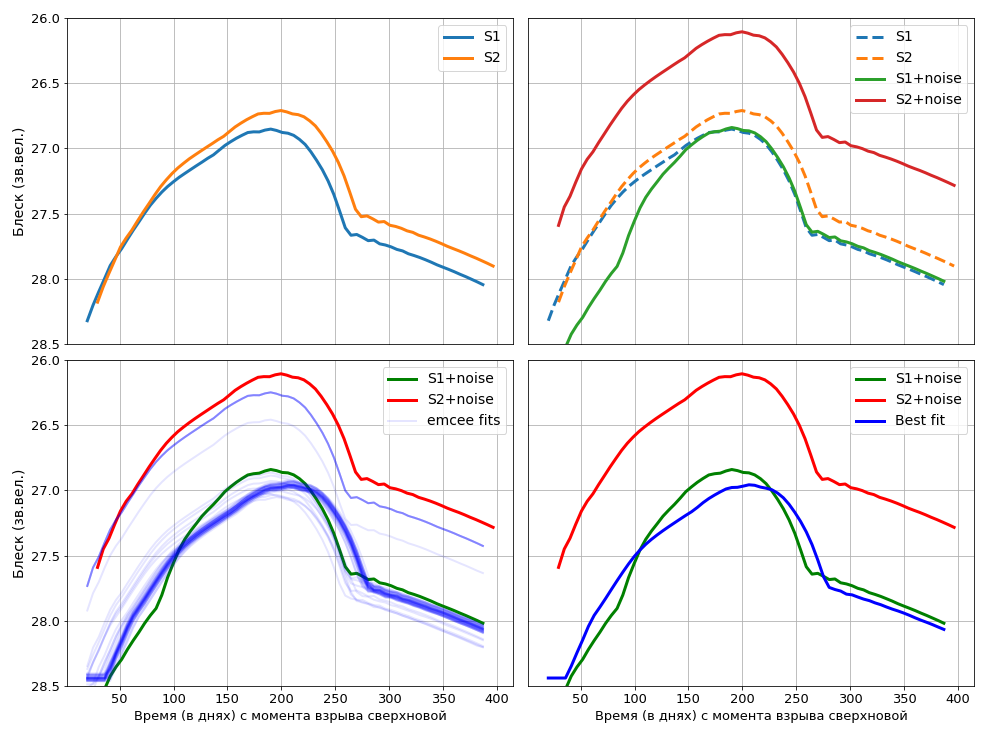
\includegraphics[width=0.99\textwidth]{microlensing/images/fitting.png}
	\caption{Сверху слева: рассматриваются кривые блеска SN Refsdal, наблюдаемые в изображениях S1 и S2. Сверху справа: одна из реализаций прибавления шума от микролинзирования к кривым блеска (в данном случае форма кривой блеска в изображении S1 в первые 150 дней сильно искажается, а вот кривая в изображении S2 всего лишь сдвигается, испытывая одинаковое смещение во всех точках). Снизу слева: различные реализации алгоритма аппроксимации. Снизу справа: "зашумленные" \ кривые блеска и наилучшая аппроксимация.  } 
	\label{fig:lc}
\end{figure}

На левой нижней панели Рисунка \eqref{fig:lc} изображены $100$ фитов, для каждого из которых вычисляется функция правдоподобия, определяемая выражением

%\begin{equation}
%\log p = -\frac{1}{2} \sum \big( m_{S1} - m_{S1}^{fit} \big)^2 \rightarrow \max 
%\end{equation}

\begin{equation}\label{eq:logprob}
\log p = -\frac{1}{2} \sum \frac{( m_{S1} - m_{S1}^{fit} )^2}{\sigma_m^2} + \log \big( 2\pi\sigma_m^2 \big).
\end{equation}

\noindent Cуммирование подразумевается по всем точкам на кривой блеска. Из всех кривых $m_{S1}^{fit}$ выбирается та, для которой функция правдоподобия максимальна (Рис. \eqref{fig:lc}, справа снизу). Непосредственно для этой реализации получается: $$\Delta t_{best} = -8.6 \ \textrm{дней}, \ \ \ \Delta m_{best} = -0.84$$ Видно, что данные значения сильно отличаются от значений ${\Delta t_{21}}^{true}$ и ${\Delta m_{21}}^{true}$. 







